\documentclass[
10pt, % Set the default font size, options include: 8pt, 9pt, 10pt, 11pt, 12pt, 14pt, 17pt, 20pt
%
aspectratio=169, % Uncomment to set the aspect ratio to a 16:9 ratio which matches the aspect ratio of 1080p and 4K screens and projectors
]{beamer}

\usepackage{xcolor,colortbl}
\usepackage{booktabs}
\usefonttheme[onlymath]{serif} 
\usetheme[progressbar=frametitle]{metropolis}
\usepackage{appendixnumberbeamer}
\usepackage{graphicx,calc}
\newlength\myheight
\newlength\mydepth
\settototalheight\myheight{Xygp}
\settodepth\mydepth{Xygp}
\setlength\fboxsep{2pt}
\newcommand*\inlinegraphics[1]{%
	\settototalheight\myheight{Xygp}%
	\settodepth\mydepth{Xygp}%
	\raisebox{-\mydepth}{\includegraphics[height=\myheight]{#1}}%
}
\usepackage{booktabs}
\usepackage[scale=2]{ccicons}

\usepackage{pgfplots}
\usepgfplotslibrary{dateplot}

\usepackage{xspace}
\newcommand{\themename}{\textbf{\textsc{metropolis}}\xspace}

\usepackage[utf8]{inputenc}
\usepackage{pifont}
\usepackage{caption}
\usepackage{xcolor}
\usepackage{animate}
\usepackage{amsmath}
\usepackage{amssymb}
\usepackage{amsfonts}
\usepackage{verbatim}
\usepackage{amsthm}
\usepackage{geometry}
\usepackage{hyperref} %Références cliquables
\usepackage{cleveref}
\usepackage{csquotes}
\usepackage{mathtools}
\usepackage{relsize}
\usepackage{tcolorbox}
\usepackage{tikz}
\usepackage{fontawesome5}
\usepackage{academicons}
\usetikzlibrary{snakes,arrows,shapes}
%%%%%%%%%%%%%%%%%%%%%%%%%%%%%%%%%%%%%%%%%%%%%%%%%%%%%%%%%
\definecolor{gold}{rgb}{0.83, 0.69, 0.22}
\definecolor{gamboge}{rgb}{0.89, 0.61, 0.06}
\definecolor{aliceblue}{rgb}{0.94, 0.97, 1.0}
\definecolor{ballblue}{rgb}{0.13, 0.67, 0.8}
\definecolor{charcoal}{rgb}{0.21, 0.27, 0.31}
\definecolor{lightkhaki}{rgb}{0.94, 0.9, 0.55}
\definecolor{applegreen}{rgb}{0.55, 0.71, 0.0}
\definecolor{ao}{rgb}{0.0, 0.5, 0.0}
\definecolor{aureolin}{rgb}{0.99, 0.93, 0.0}
\definecolor{awesome}{rgb}{1.0, 0.13, 0.32}
\definecolor{amaranth}{rgb}{0.9, 0.17, 0.31}
\definecolor{almond}{rgb}{0.94, 0.87, 0.8}
\definecolor{mintgreen}{rgb}{0.6, 1.0, 0.6}
\definecolor{palatinatepurple}{rgb}{0.41, 0.16, 0.38}
\definecolor{oldlace}{rgb}{0.99, 0.96, 0.9}
\definecolor{lavendermist}{rgb}{0.9, 0.9, 0.98}
	\definecolor{dimgray}{rgb}{0.41, 0.41, 0.41}
\setbeamercolor{block title}{use=structure,fg=amaranth,bg=lavendermist}
\setbeamercolor{block body}{use=structure,fg=black,bg=oldlace}
\setbeamercolor{frametitle}{fg=white,bg=black}
\setbeamercolor{progress bar}{fg=amaranth,bg=white}
\setbeamercolor*{structure}{bg=white,fg=amaranth}
\setbeamercolor{block title alerted}{fg=white,bg=amaranth}
%body
\setbeamercolor{block body alerted}{fg= black,bg=almond}

\newenvironment{variableblock}[3]{%
	\setbeamercolor{block body}{#2}
	\setbeamercolor{block title}{#3}
	\begin{block}{#1}}{\end{block}}

%%%%%%%%%%%%%%%%%%%%%%%%%%%%%%%%%%%%%%%%%%%%%%%%%%%%%%%%%%5
\theoremstyle{plain}% default
\newtheorem{thm}{Theorem}[section]
\newtheorem{lem}[thm]{Lemma}
\newtheorem{prop}[thm]{Proposition}
\newtheorem*{cor}{Corollary}
\theoremstyle{definition}
\newtheorem{defn}{Definition}[section]
\newtheorem{exmp}{Example}[section]
\newtheorem{xca}[exmp]{Exercise}
\theoremstyle{remark}


%--------------- Commands

%------------Commands-----------%
\newcommand{\calA}{\mathcal{A}}
\newcommand{\calB}{\mathcal{B}}
\newcommand{\calS}{\mathcal{S}}
\newcommand{\calP}{\mathcal{P}}
\newcommand{\calH}{\mathcal{H}}
\newcommand{\calL}{\mathcal{L}}
\newcommand{\calC}{\mathcal{C}}
\newcommand{\calD}{\mathcal{D}}
\newcommand{\calO}{\mathcal{O}}
\newcommand{\calR}{\mathcal{R}}
\newcommand{\calT}{\mathcal{T}}
\newcommand{\calX}{\mathcal{X}}
\newcommand{\fqm}{\mathbb{F}_{q^m}}
\newcommand{\fq}{\mathbb{F}_{q}}
\newcommand{\fqo}{\mathbb{F}_{q_0^2}}
\newcommand{\F}{\mathbb{F}}
\newcommand{\Z}{\mathbb{Z}}
\newcommand{\PP}{\mathbb{P}}
\newcommand{\R}{\mathbb{R}}
\newcommand{\Tr}[1]{\operatorname{Tr}_{}\left(#1\right)}
\newcommand{\set}[1]{\left\{#1\right\}}
\newcommand{\Floor}[1]{\left\lfloor #1 \right\rfloor}
\newcommand{\Span}[1]{\operatorname{Span}\left\lbrace #1\right\rbrace }
\newcommand{\LT}[1]{\operatorname{LT}\left(#1\right)}
\newcommand{\Supp}{\operatorname{Supp}}
\newcommand{\Div}{\operatorname{Div}}
\newcommand{\ssag}[1]{\operatorname{\mathsf{SSAG}}_{q}\left(#1\right)}
\newcommand{\GRS}{\operatorname{\mathsf{GRS}}}
\newcommand{\gen}{\mathfrak{g}}
\newcommand{\degab}[1]{\deg_{a,b}\left(#1\right)}
%%%%%%%%%%%%%%%%%%%%%%%%%%%%%%%%%%%%%%%%%%%%%%%%%%%%%%
\newcommand\myeq{\mathrel{\stackrel{\makebox[0pt]{\mbox{\normalfont\tiny def}}}{=}}}
\newcommand\scalemath[2]{\scalebox{#1}{\mbox{\ensuremath{\displaystyle #2}}}}
\setbeamertemplate{frametitle}{%
	\nointerlineskip%
	\begin{beamercolorbox}[wd=\paperwidth,ht=2.0ex,dp=0.6ex]{frametitle}
		\hspace*{1ex}\insertframetitle%
	\end{beamercolorbox}%
}
\makeatletter



\vfuzz=25pt %Evite les alertes "Over full \vbox" jusqu'à 25pt.

%---------------- Tikz Packages ------------------
\usepackage{tikz}
\usetikzlibrary{tikzmark} %Permet de créer des noeuds dans du texte pour annoter dans un tikz ultérieur. Très pratique pour annoter les formules moches.
\usetikzlibrary{arrows,patterns,positioning,fit}
\usetikzlibrary{matrix,arrows,shapes,shapes.misc}
\usetikzlibrary{decorations.pathreplacing,angles,quotes}
\usetikzlibrary{decorations.markings,calc}
\usetikzlibrary{overlay-beamer-styles,backgrounds} %Pour utiliser alt dans tikz
\tikzset{>=stealth} % Change le style de flèche dans tikz

%--------- Un bout de code pour récupérer la couleur d'un noeud rectangulaire ou circulaire : noeud.f pour la couleur du fill, noeud.d pour celle du draw ---------------
% Voir https://tex.stackexchange.com/questions/602047/is-obtaining-the-color-of-a-node-possible

\makeatletter
\def\pgf@sh@fbg@circle{%
	\@ifundefinedcolor{pgffillcolor}{}{\xglobal\colorlet{\pgf@node@name.f}{pgffillcolor}}%
	\@ifundefinedcolor{pgfstrokecolor}{}{\xglobal\colorlet{\pgf@node@name.d}{pgfstrokecolor}}%
}
\def\pgf@sh@fbg@rectangle{%
	\@ifundefinedcolor{pgffillcolor}{}{\xglobal\colorlet{\pgf@node@name.f}{pgffillcolor}}%
	\@ifundefinedcolor{pgfstrokecolor}{}{\xglobal\colorlet{\pgf@node@name.d}{pgfstrokecolor}}%
}
\makeatother

%-Après avoir défini un \tikzmarknode{noeuf}{texte}, on crée un noeuf rectangulaire (aux coins arrondis) autour d'une certaine couleur et on annote avec une flèche.

\newcommand\highlightnode[2]{ %args: noeud, couleur
	\node (#1-frame)[rounded corners,fit=(#1),inner sep=2pt,fill=#2,fill opacity=0.17] {};
}

\newcommand\framenode[6][(0,0)]{ %args: (shift) noeud, position, couleur, texte , booléen flèche 0 = non / 1 = oui
	\highlightnode{#2}{#4}
	\node [#2-frame.f,#3 of = #2, shift={#1}](#2-text){#5};
	\ifx1#6 	\draw[#2-frame.f,<-] (#2-frame) -- (#2-text); \fi		
}


%%%%%%%%%%%%


\usepackage[symbol]{footmisc}
\renewcommand{\thefootnote}{\fnsymbol{footnote}}

%%%%%%%%%%%%%%%%%%%%%%%%%%%% Title %%%%%%%%%%%%%%%%%%%%%
\title[Goppa-Like AG codes Distinguisher]{Goppa–Like AG Codes On $C_{a,b}$ Curves}
%\subtitle{Subtitle}
\author[SEK]{\textbf{Sabira El Khalfaoui} \vspace{0.3cm}\\\vspace{1cm} \textit{\textcolor{amaranth}{Joint work with}} \textbf{Mathieu Lhotel, Jade Nardi}}


\institute[]{\large{\textbf{Journ\'ee de} \\ \smallskip \textit{\textcolor{amaranth}{l'IRMAR}\\ \vspace{-0.3em}\textbf{30 mai 2023}}}}
\date[Mai 2023]

\begin{document}
	
	\maketitle
	
	\begin{frame}{Table of contents}
		\setbeamertemplate{section in toc}[sections numbered]
		\tableofcontents%[hideallsubsections]
	\end{frame}
	
	\section{Code-based cryptography}
	\begin{frame}
		\frametitle{Error-correcting codes}
		Let $q$ be a prime power and $m \geq 1$. 
		\begin{block}{Definition: Linear code}
			A \textbf{linear code} $\calC$ of length $n$ over $\fq$ is a vector subspace of $\fq^n$.
		\end{block}
	\begin{block}{Reed-Solomon code}
		Let $\mathbf{x}=(x_1,\cdots,x_n) \in \fq^n$ with distinct entries, the \textbf{Reed-Solomon code} is defined as
		\vspace{-0.7em}
		$$RS_r(\mathbf{x})=\{(f(x_1),f(x_2),\dots,f(x_n)) \mid f \in \fq[X] \text{ such that } \deg f < r \}.$$
	\end{block}
		\begin{block}{Definition: Dual code}
			The \textbf{dual code} $\calC^{\perp}$ of $\calC$ is defined by 
		$\calC^{\perp}=\left\lbrace \mathbf{x} \in \fq^n \mid \mathbf{c} \cdot \mathbf{x}=0, \text{ for all } \mathbf{c} \in \calC \right\rbrace,$
			where $(\cdot)$ is the usual scalar product.
		\end{block}
%		\vspace{-0.7em}
		\begin{tcolorbox}[colback=white,colframe=palatinatepurple]
			A \textbf{generator matrix} for a linear code $\calC$ is a matrix $G$ whose rows form a basis for $\calC$.
		\end{tcolorbox}
		
	\end{frame}
	\begin{frame}
		\frametitle{Difficult Problem}
		\begin{block}{Definition: Hamming weight}
			The \textbf{Hamming weight} of $x \in \fq^n$ is defined by:
			$w(x)\myeq \# \left\lbrace i \in \{1,\dots,n\} \, | x_i\neq 0\right\rbrace.$
		\end{block}
		\begin{alertblock}{Difficult problem - Bounded decoding problem }
			Given an linear code $\calC \subseteq \fq^n $, $y\in \fq^n$ and $t \geq 0$. Does there exist $c \in \calC$ such that
		
			\[w(y-c) \leq t ?\]
			It is an \textit{NP-Complete} problem (Berlekamp, McEliece, Van Tilborg 1978).
		\end{alertblock}
		A \textbf{t-decoder} for $\calC$ is an algorithm $\calA$:
		\begin{itemize}
		
			\item \textbf{Input:} $y\in \fq^n$.
			\item \textbf{Output:} $ c\in \calC$ such that  $w(y-c)\leq t $ if exists.
		\end{itemize}
	\end{frame}
	\begin{frame}
		
		\frametitle{McEliece cryotosystem}
		\textbf{McEliece} introduced the first public key cryptosystem based on error-correcting codes in 1978.
		
		\begin{itemize}
		 \item \textcolor{amaranth}{\textbf{Secret Key:}} A generator matrix $G$ of a linear code $\calC$ having an efficient $t-$decoding algorithm $\calA_{\calC}$.
		 \item \textcolor{amaranth}{\textbf{Public Key:}} $G'= SGP$, where $S$ is a $k\times k$ invertible matrix and $P$ is an $n\times n$ permutation matrix.
		 \item \textcolor{amaranth}{\textbf{Encryption:}} $m \in \fq^k\,\,$ \textrightarrow $\,\,y=mG'+ e$, where $e $ is a random error of weight $t$.
		 \item \textcolor{amaranth}{\textbf{Decryption:}} $yP^{-1}=mSG+eP^{-1}$, then we decode to get $mS$. Thus $mSS^{-1}=m$.
		\end{itemize}
		
%		\begin{itemize}
%			\item McEliece introduced the first public key cryptosystem based on error-correcting codes in 1978.
%			\item Let $\mathbf{\mathcal{F}}$ be any family of linear codes $\calC$ with an efficient $t-$decoding algorithm $\calA_{\calC}$ where each element is represented by the triple $(\calC, \calA_{\calC}, t)$.
%		\end{itemize}
		%\vspace{-0.7em}
		\begin{columns}[T,onlytextwidth]
			\column{0.5\textwidth}
%			\begin{block}{\textit{\textbf{Key Generation}}}
%				Given an element $(\calC, \calA_{\calC}, t) \in \mathcal{F}$:
%				\vspace{-0.7em}
%				\begin{dinglist}{52}
%					\item 
%					\item $G$ non-structured \textbf{generator matrix} of $\calC$.
%				\end{dinglist}
%				\vspace{-0.7em}
%				\begin{itemize}
%					\item[\textcolor{palatinatepurple}{\textrightarrow}] \textcolor{palatinatepurple}{\textbf{McEliece Public Key:}} $\mathcal{K}_{pub}=(\mathbf{G}, t)$.
%					\item[\textcolor{amaranth}{\textrightarrow}] \textcolor{amaranth}{\textbf{McEliece Secret Key:}} $\mathcal{K}_{secret}= (\calA_{\calC})$.
%				\end{itemize}
%			\end{block}
			\textcolor{palatinatepurple}{\textbf{\textit{Advantages:}}}
			\begin{dinglist}{52}
				\item Post-quantum cryptography.
				\item Fast encryption and decryption functions.
			\end{dinglist}
			\column{0.5\textwidth}
%			\begin{variableblock}{\textbf{\textit{Encryption}}}{bg=almond,fg=black}{bg=palatinatepurple,fg=white} Encrypt $\mathbf{m} \in \fq^k$ as 
%				\vspace{-0.9em}
%				$$\mathbf{mG} +e $$ where $e $ is a random error of weight $t$.
%				
%			\end{variableblock}
%			\vspace{-0.7em}
%			\begin{alertblock}{\textbf{\textit{Decryption}}}
%				Apply $\calA_{\calC}$ to $\mathbf{mG}+e$ to recover $mathbf{m}$.
%			\end{alertblock}
			\textcolor{amaranth}{\textbf{\textit{Drawback:}}}
			\begin{itemize}
				\item[\color{amaranth}{\ding{55}}] Large key size
			\end{itemize}
		\end{columns}
		\vspace{0.3em}
		\textcolor{palatinatepurple}{\faIcon{file-alt}}  \textbf{McEliece's original proposal} (McEliece 1978) is based on \textbf{binary Goppa code}. 
		
		%\textcolor{amaranth}{\textrightarrow Large key size} .
	\end{frame}
	\section{AG codes on algebraic curves}
	
	%%%%%%%%%%%%%%%%%%%%%%%%%%%%%
	\begin{frame}
		\frametitle{Agebraic Geometry (AG) codes}
		\vspace{1em}
		\begin{columns}
			
			\hspace{-20pt}
			\column{0.5\textwidth}
			%\vspace{0.5em}
		\textbf{\textcolor{palatinatepurple}{Reed-Solomon code}}:
		\vspace{-0.9em}
			\begin{center}
				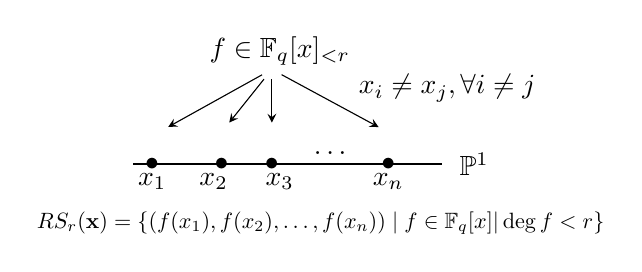
\begin{tikzpicture}[scale=0.8]
					%\node (T) at (-2.4,2.5) {\textbf{Reed-Solomon code:}};
					\node (A) at (-2.4,-0) {};
					\node (B) at (2.5,0) {};
					\node (C) at (-.2,1.5) {};
					\node (D) at (-2,0.5) {};
					\node (E) at (-1,0.5) {};
					\node (F) at (-0.2,0.5) {};
					\node (G) at (1.65,0.5) {};
					%Points
					
					\node[label={[label distance=-2mm]below:$x_1$}] (P1) at  (-2.1,0) {$\bullet$};
					\node[label={[label distance=-2mm,xshift=-0.1cm]below:$x_2$}] (P2) at (-1,0) {$\bullet$};
					\node[label={[label distance=-2mm,xshift=0.1cm]below:$x_3$}] (P3) at (-.2,0) {$\bullet$};
					\node[label={[label distance=-2mm]below:$x_n$}] (Pn) at  (1.65,0) {$\bullet$};
					
					\path (P3) to node[sloped, midway,above,black] {$\mathbf{\dots}$} (Pn) ;
					
					%Courbe
					\node[right=0.1cm] at  (0.9,1.2) {$x_i\neq x_j, \forall i\neq j$};
					\node[right=0.1cm] at  (B) {$\mathbb{P}^1$};
					\draw[thick] plot [smooth] coordinates {(A) (P1) (P2) (P3) (Pn) (B)};
					\node [label={[label distance=-2mm,xshift=0.1cm]above:$f \in \mathbb{F}_q[x]_{<r}$}] at (-.2,1.5) {} ;
					%\draw[white] (1,.9) rectangle (2,1.1);
					\draw[-stealth] (C)--(D);
					\draw[-stealth] (C)--(E);
					\draw[-stealth] (C)--(F);
					\draw[-stealth] (C)--(G);
					\node[label={[label distance=-2mm,xshift=-0.1cm]below:\scalemath{0.8}{RS_r(\mathbf{x})=\{(f(x_1),f(x_2),\dots,f(x_n)) \mid f \in \fq[x]| \deg f < r \}}}] at (0.7,-0.7) {} ;
					%\node (TT) at (-0.3,-1,2) {\textbf{Generalized Reed-Solomon code:}};
				\end{tikzpicture}
			\end{center}
			\vspace{-0.7em}
			\textbf{\textcolor{palatinatepurple}{AG code on the curve $\calX$ over $\fq$}}
			\vspace{-0.7em}
			\begin{center}
				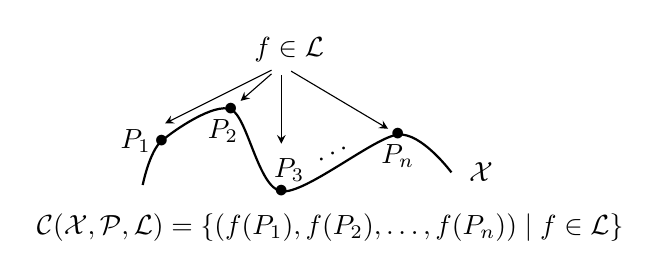
\begin{tikzpicture}[scale=0.8]
					%\node (T) at (-2.4,2.5) {\textbf{Reed-Solomon code:}};
					\node (A) at (-2.4,-0) {};
					\node (B) at (2.5,0) {};
					\node (C) at (-.2,1.7) {};
					\node (D) at (-2.2,0.7) {};
					\node (E) at (-1,1) {};
					\node (F) at (-0.2,0.3) {};
					\node (G) at (1.65,0.6) {};
					%Points
					
					\node (A) at (-2.4,-0.2) {};
					\node (B) at (2.5,0) {};
					
					%Points
					
					\node[label={[label distance=-2mm]left:$P_1$}] (P1) at  (-2.1,0.5) {$\bullet$};
					\node[label={[label distance=-2mm,xshift=-0.1cm]below:$P_2$}] (P2) at (-1,1) {$\bullet$};
					\node[label={[label distance=-2mm,xshift=0.1cm]above:$P_3$}] (P3) at (-.2,-0.3) {$\bullet$};
					\node[label={[label distance=-2mm]below:$P_n$}] (Pn) at  (1.65,0.6) {$\bullet$};
					
					\path (P3) to node[sloped, midway,above,black] {$\dots$} (Pn) ;
					
					%Courbe
					
					%\node[right=0.1cm] at  (0.6,1.5) {$\calP=\{P_1,P_2,\cdots,P_n\}$};
					\node[right=0.1cm] at  (B) {$\calX$};
					\draw[thick] plot [smooth] coordinates {(A) (P1) (P2) (P3) (Pn) (B)};
					\node [label={[label distance=-2mm,xshift=0.1cm]above:$f \in \calL$}] at (-.2,1.7) {} ;
					%\draw[white] (1,.9) rectangle (2,1.1);
					\draw[-stealth] (C)--(D);
					\draw[-stealth] (C)--(E);
					\draw[-stealth] (C)--(F);
					\draw[-stealth] (C)--(G);
					\node[label={[label distance=-2mm,xshift=-0.1cm]below:\scalemath{1}{\mathcal{C}(\mathcal{X}, \mathcal{P},\calL)=\{(f(P_1),f(P_2),\dots,f(P_n)) \mid f \in \calL \}}}] at (0.7,-0.6) {} ;
					%\node (TT) at (-0.3,-1,2) {\textbf{Generalized Reed-Solomon code:}};
				\end{tikzpicture}
			\end{center}
			\hspace{-30pt}
			\column{0.5\textwidth}
			\vspace{-4em}
			\begin{block}{\textbf{Generalized Reed--Solomon (GRS)}}
				Let $\mathbf{x}\in \fq^n$  with distinct entries (\textbf{support}) and \textbf{multiplier} $\mathbf{y} \in (\fq^*)^n$.
				\vspace{-0.7em}
				\begin{align*}
					\GRS_r(\mathbf{x}, \mathbf{y})=&\{(y_1f(x_1),y_2f(x_2),\dots,y_nf(x_n))\\
					& \mid f \in \fq[X] \text{ such that } \deg f < r \}.
				\end{align*}
			\end{block}
%\vspace{5em}
\vspace{-0.7em}
		\begin{itemize}
			%\item The dimension of $RS_r$ is $r$,
			\item $n\leq q$.
			%\vspace{-0.7em}
		\end{itemize}
	%\vspace{0.3em}
	%$\calX$ be an algebraic curve\\
	%\vspace{3em}
	\textbf{\textcolor{amaranth}{AG code $\mathcal{C}(\mathcal{X}, \mathcal{P},\calL)$ parameters:}}\\
	%\vspace{0.3em}
	$\calP=\{P_1,P_2,\cdots,P_n\}$ is a set of distinct rational points of $\calX$.\\
		%\vspace{0.3em}
		%\vspace{1em} 
		%\vspace{0.5em}
		\begin{itemize}
			\item $k \leq \dim \calL$,
			\item $n=\# \calP$.
			\item[\color{amaranth}{\ding{52}}] $n>q$.
		\end{itemize}
		\vspace{0.5em}
		\end{columns}
	\end{frame}
	%%%%%%%%%%%%%%%%%%%%%%%%%%%%%
	
	\begin{frame}
		\frametitle{AG codes on $C_{a,b}$ curve}
		\begin{block}{Definition (Miura 1993)}
			Let $a,b$ be coprime positive integers. A $\mathbf{C_{a,b}}$ \textbf{curve} over $\fqm$ is a curve $\calX_{a,b}$ having an irreducible, affine and non--singular plane model with equation
			%\begin{equation} \label{eq:equation_C_ab}
			\vspace{-0.7em}
			\[f_{a,b}(x,y) = \alpha_{0,a}y^a + \alpha_{b,0}x^b + \sum_{ai+bj < ab} \alpha_{i,j}x^iy^j = 0\]	
			%\end{equation}
			%\vskip-1.5em %\hfill 		
			with $\alpha_{0,a}$ and $\alpha_{b,0} \neq 0$.
		\end{block}
		\vspace{-0.7em}
		Examples of $C_{a,b}$ curves: Elliptic curves, Hermitian curve...
		\vspace{-0.5em}
		\begin{itemize}
			\item Its genus is $\mathfrak{g}_{a,b}=\dfrac{(a-1)(b-1)}{2}$.
			%, and it has a unique point at infinity, denoted by $P_{\infty}$.
			%Riemann--Roch space $\calL(s P_\infty)$ has an explicit basis as follows:
			\item Define $\degab{x^iy^j}= ai+bj$, and $\degab{f}= \degab{LT(f)}$ for $f\in \fq[x,y]$.
			\item $\calL(s)= \Span{x^iy^j \mid 0 \leq i, 0\leq j\leq a-1 \ \mathrm{and} \ \degab{x^iy^j} \leq s}$.
			\item $\dim \calL(s) \geq s +1-\mathfrak{g}_{a,b}$. Equality if $s \geq 2\mathfrak{g}_{a,b} -1$.
		\end{itemize}
		\vspace{-0.5em}
		\begin{center}
		\scalebox{0.9}{
		\begin{tcolorbox}[colback=white,colframe=palatinatepurple]
			The AG code associated to $(\calX_{a,b}, \calP, \calL(s))$ is:
			\vspace{-0.9em}
			$$ \calC(\calX_{a,b},\calP,\calL(s))= \left\lbrace (f(P_1),\cdots,f(P_n))\,|\, f \in \calL(s)\right\rbrace.$$
			
		\end{tcolorbox}
	}
	\end{center}
	\end{frame}

\begin{frame}
	\frametitle{Subfield Subcodes}
	\begin{block}{Subfield subcode}
		Let $\calC$ be a linear code over $\fqm$.
		Its \textbf{subfield subcode} $\calC|_{\fq}$ is defined by 
		\vspace{-0.7em}
		\[\calC|_{\fq}=\calC \cap \mathbb{F}_q^n.\]
	\end{block}
	\begin{block}{Definition: Goppa code}
		%Let $\mathbf{x} \in \fqm^n$ be a vector with distinct entries and $g \in \fqm [x]_{<r}$ is called \textbf{Goppa polynomial} such that $\forall i, g(x_i)\neq 0$, the \textbf{Goppa code} associated to $(\mathbf{x}, g)$ is defined as:
		Let $\mathbf{x} \in \fqm^n$ be a vector with distinct entries, and let $g \in \fqm [x]_{=r}$ be referred to as the \textbf{Goppa polynomial}, satisfying $\forall i, g(x_i)\neq 0$. The \textbf{Goppa code} associated with $(\mathbf{x}, g)$ is 	
		\vspace{-0.7em}
		 \[\Gamma_r(\mathbf{x},g)= \GRS_r(\mathbf{x},g(\mathbf{x})^{-1})^\perp|_{\fq},\]
		where $g(\mathbf{x})^{-1}=(g(\mathbf{x_1})^{-1},\dots,g(\mathbf{x_n})^{-1})$
	\end{block}
\begin{tcolorbox}[colback= white, colframe=palatinatepurple]
	The subfield subcode (\textbf{SSAG}) of an AG code $C(\calX,\calP,\calL)$ defined over $\fqm$ is
	\[C(\calX,\calP,\calL)|_{\fq}.\]
\end{tcolorbox}
\end{frame}
	
	%%%%%%%%%%%%%%%%%%%%%%%%%%%%%%%%%%%%%%%%%%%%%%%%%%%%%%%%%%%%%%%
	\section{McEliece cryptosystem - Variants (Motivation I)}
	\begin{frame}
		\frametitle{McEliece Cryptosystem - Variants}
		The \textbf{security} of \textbf{McEliece cryptosystem} is based on:
		\begin{itemize}
			\item the hardness of \textbf{decoding} random linear codes,
			\item the \textbf{indistinguishability} of the chosen codes from random ones.
		\end{itemize}
		
		%\vspace{0.5em}
		
		%\textcolor{applegreen}{\faCheckCircle} It is still resistant to attack. \textcolor{red}{\faExclamationTriangle} Large key size.
		\textcolor{palatinatepurple}{\textbf{How To Reduce The Key Size?}}
		
		\begin{columns}[T,onlytextwidth]
			\column{0.6\textwidth}
			\begin{itemize}
				\item[\textcolor{palatinatepurple}{\faIcon{file-alt}}] \textbf{GRS} codes with $m = 1$ by \textbf{Niederreiter} 1986.
				\item[\textcolor{amaranth}{\faFrownOpen}] Broken by
				\textbf{Sidelnikov and Shestakov}.
				\item[\textcolor{palatinatepurple}{\faIcon{file-alt}}] \textbf{AG codes} and \textbf{\textcolor{applegreen}{SSAG}} by \textbf{Janwa, Moreno} 1996.
				\item[\textcolor{amaranth}{\faFrownOpen}]\textbf{ AG codes} for genus $\leq 2$ is broken by \textbf{Faure Minder} 2008. For any genus by \textbf{Couvreur, Marquez–Corbella, Pellikaan} 2014 - 2017.
			\end{itemize}
			\column{0.4\textwidth}
			\begin{enumerate}
				\item[\textcolor{palatinatepurple}{\faIcon{file-alt}}] \textbf{Subcodes} of \textbf{GRS codes} by \textbf{Berger, Loidreau} 2001.
				\item[\textcolor{amaranth}{\faFrownOpen}] Broken by \textbf{Wieschebrink} 2010.
				\item[\textcolor{applegreen}{\faIcon{file-alt}}] In (E.K, Nagy 2021) we suggest "the $\mathbb{F}_{q^2}/\fq$ \textbf{subfield subcodes} of $1$\textbf{-point Hermitian codes}".
			\end{enumerate}
		\end{columns}
		\vspace{0.3em}
		\begin{tcolorbox}[colback=white,colframe=palatinatepurple]
			\textcolor{applegreen}{\faIcon{file-alt}} In this work we propose to use \textbf{Goppa-like AG codes on $C_{a,b}$ curves}.
		\end{tcolorbox}
	\end{frame}
	
	
	\begin{frame}
		\frametitle{Classical Goppa code VS Goppa-like AG code construction }
		
		\begin{columns}[T]
			%\hspace{-10pt}
			\column{0.5\textwidth}
		\textcolor{amaranth}{\textbf{Classical Goppa code}}
		\begin{itemize}
			\item The projective line $\mathbb{P}^1$ over $\fqm$,
			\item $\fqm[x]_{<r}$,
			%\vspace{1em}
			\item $g \in \fqm[x]_{= r}$,
			%\vspace{0.5em}
			\item $\mathbf{x}=(x_1,\cdots,x_n)$,
			%\vspace{0.5em}
			\item $\forall i, g(x_i)\neq 0$,
			%\vspace{0.5em}
			\item $\GRS_r(\mathbf{x}, g(\mathbf{x})^{-1})$,
			\textcolor{amaranth}{$(g(x_1)^{-1}f(x_1),\dots,g(x_n)^{-1}f(x_n)) $.}
		\end{itemize}
		\begin{block}{Classical Goppa codes}
			$$\Gamma_r(\mathbf{x},g)= \GRS_r(\mathbf{x},g(\mathbf{x})^{-1})^\perp|_{\fq}$$
		\end{block}
			%\hspace{-30pt}
			\column{0.6\textwidth}
				\textcolor{palatinatepurple}{\textbf{Goppa-like AG code}}
			\begin{itemize}
				\item[\textcolor{palatinatepurple}{\faArrowCircleRight}] A $C_{a,b}$ curve $\calX_{a,b}$ over $\fqm$, %\textcolor{palatinatepurple}{\faArrowCircleRight}
				\item[\textcolor{palatinatepurple}{\faArrowCircleRight}] The v.s $\calL(s)$ of functions $f$ where $\degab{f} \leq s$, 
				%on the curve $\calX_{a,b}$ %\textcolor{palatinatepurple}{\faArrowCircleRight}
				\item[\textcolor{palatinatepurple}{\faArrowCircleRight}] Let $g $ such that $\degab{g}=s'$ with $s'>s$, %\textcolor{palatinatepurple}{\faArrowCircleRight}
				\item[\textcolor{palatinatepurple}{\faArrowCircleRight}] $\calP= \{P_1,P_2,\cdots,P_n\}$, %\textcolor{palatinatepurple}{\faArrowCircleRight}
				\item[\textcolor{palatinatepurple}{\faArrowCircleRight}] $\forall i$, $g(P_i)\neq 0$,
				\item[\textcolor{palatinatepurple}{\faArrowCircleRight}] $\calC=\calC(\calX_{a,b},\calP,g^{-1}\calL(s))$, %\textcolor{palatinatepurple}{\faArrowCircleRight}.
				\textcolor{palatinatepurple}{ $\left( g^{-1}(P_1)f(P_1),\dots,g^{-1}(P_n)f(P_n) \right)$.}
			\end{itemize}
			\begin{block}{The \textbf{Goppa--like} AG code associated to $\calC$}
				$$ \Gamma(\calX_{a,b},\calP,g) := \calC^{\perp}|_{\fq}.$$
			\end{block}
			
		\end{columns}
		
	\end{frame}
	\begin{frame}
		\frametitle{Motivation I: McEliece Cryptosystem - New Variants}
		\textbf{\textcolor{amaranth}{Variants based on Subfield Subcodes of AG codes}}
		\begin{table}[h]
			\begin{center}
				\scalebox{0.8}{
					\begin{tabular}{|c|c|c|c|c|c|c|}
						\hline
						$q$&  $s$ & $n$ & $k$ & $t$ & Security bits\footnote{\textbf{With respect to Prange algorithm}}& Key--Size(bit)\\
						\hline \hline
						
						${11}$	&1\,174 & 1\,331 & 927 & 78 & $142$ & $1\,123\,524$ \\
						
						\hline \hline
						${13}$&2\,039 & 2\,197 & 1\,735 & 79 & $185$ & $3\,206\,280$ \\
						
						\hline 
						${16}$&3\,980 & 4\,096 & 3\,634 & 58 & 187& 6\,715\,632   \\
						
						\hline \hline
						${13}$& 1\,861 & 2\,197 & 1\,398 & 168 & 263& 4\,468\,008\\
						
						\hline 
						${16}$& 3\,874 & 4\,096 & 3\,422 & 111 & 300 & 9\,225\,712\\
						\hline
				\end{tabular}}
				%\vspace*{0.1em}
				\caption{McEliece cryptosystem based on \textbf{1-point Hermitian subfield subcodes }(E.K, Nagy 2021).}
			\end{center}
		\end{table}
		\vspace*{-0.8em}
		\begin{table}[h]
			\begin{center}
				\scalebox{0.8}{
					\begin{tabular}{|c|c|c|c|c|c|c|}
						\hline
						$q$&  $s$ & $n$ & $k$ & $t$ & Security bits& Key--Size(bit)\\
						\hline \hline
						
						${11}$	&265&1320& 898& 77& \cellcolor{almond}\textbf{153}& 1\,136\,868 \\
						
						\hline \hline
						\rowcolor{almond} \textbf{13}&\textbf{312}&\textbf{2188}& \textbf{1718}& \textbf{77}& \textbf{198}& \textbf{2\,422\,380}  \\
						
						\hline 
						${16}$&354& 4078& 3608& 56& \cellcolor{almond}\textbf{199}& 6\,783\,040   \\
						
						\hline \hline
						\rowcolor{almond}\textbf{13}& \textbf{490}& \textbf{2189}& \textbf{1363}& \textbf{166}& \textbf{270}& \textbf{3\,377\,514} \\
						
						\hline 
						${16}$& 460 &4080& 3398& 109& \cellcolor{almond}\textbf{313}& 9\,269\,744\\
						\hline
				\end{tabular}}
				%\vspace*{0.1em}
				\caption{\textbf{Goppa-Like Hermitian codes }parameters $\Gamma(\calP,sP_\infty,g)$ over $\F_{q^2}$ (E.K, Lhotel, Nardi 2023).} \label{table:goppa-herm}
			\end{center}
		\end{table}
		\vspace*{-0.8em}
	\end{frame}
	\section{Schur product - Square code - Distinguisher (Motivaton II)}
	%-----------------------------------------
	\begin{frame}
		\frametitle{Schur Product and Square code Distinguisher}
		In $\fq^n$ we denote by $\star$ the \textbf{Schur product}:
		\[ \mathbf{c} \star \mathbf{d} \myeq (c_1d_1,\cdots,c_nd_n). \]
		%	\begin{block}{Definition: Schur product}
			%		The Schur product of two vectors $\mathbf{a}$,$\mathbf{b} \in \fqm^n$ is defined as 
			%		\[ \mathbf{a} \star \mathbf{b} := (a_1b_1,\cdots,a_nb_n). \]
			%	\end{block}
		A linear code $\calC \subseteq \fq^n$ of dimension $k$ can be represented as:
		\[\calC =\Span{c_1,\cdots,c_k},\]
		then, the \textbf{Schur suqare} of $\calC$ is:
		\[ \mathbf{\calC } \star \mathbf{\calC }\myeq \calC^{\star2} = \Span{\mathbf{c}_i \star \mathbf{c}_j, 1\leq i \leq j \leq k}. \]
		\vspace{-0.7em}
		%	\begin{block}{Schur Product of codes}
			%		If $\calC$ and $\calD$ are two codes over $\fqm$ with same length $n$, their Schur product is defined as the following component--wise product:
			%		\[ \calC \star \calD := \Span{\mathbf{c} \star \mathbf{d} \mid \mathbf{c} \in \calC, \mathbf{d} \in \calD}. \]
			%	\end{block}
		\vspace{-0.7em}
		\begin{alertblock}{Distinguisher-Square code}
			Let $\calC\subseteq\fq^n$ be a linear code of dimension $k$, we have
			\[\displaystyle \dim (\calC^{\star2})\leq \mathcolor{amaranth}{\mathrm{min}\left(n,\binom{k+1}{2}\right)}.\]
			With a high probability, we have equality when $\calC$ is a \textcolor{amaranth}{\textbf{random code}}.
		\end{alertblock}
		We can use this property to identify certain linear codes from random ones.
		
	\end{frame}
	\begin{frame}
		\frametitle{Schur square of evaluation codes}
		\begin{block}{Definition: \textbf{Generalized Reed--Solomon (GRS)}}
			Let $\mathbf{x}\in \fq^n$ be a vector with distinct entries (\textbf{support}) and \textbf{multiplier} $\mathbf{y} \in (\fq^*)^n$.
			\vspace{-0.7em}
			\[\GRS_r(\mathbf{x},\mathbf{y})=\{(y_1f(x_1),y_2f(x_2),\dots,y_nf(x_n)) \mid f \in \fq[X] \text{ such that } \deg f < r \}.\]
		\end{block}
		\begin{block}{Schur square of $\GRS$}
			If $r \leq \frac{n+1}{2}$: then
			\vspace{-0.7em}
			$$\dim(\GRS_r(\mathbf{x},\mathbf{y})^{\star 2})=\dim(\GRS_{2r-1}(\mathbf{x},\mathbf{y\star y}))= 2r-1 < \binom{r+1}{2}.$$
		\end{block}
	\pause
		\begin{alertblock}{Schur square of AG codes on $C_{a,b}$ curve}
			Let $\calL(s)$ be a vector space of functions $f$ on $\calX_{a,b}$ such that $\degab{f}\leq s$, then
			\vspace{-0.5em}
			\[\calC(\calX_{a,b},\calP,\calL(s))^{\star 2 }\subseteq \calC(\calX_{a,b},\calP,\calL(2s)).\]
			Equality holds if $ s \geq 2\mathfrak{g}_{a,b}+1$.
		\end{alertblock}
	\vspace{-0.5em}
		\begin{itemize}
			\item [$\Longrightarrow$] For $ s \geq 2\mathfrak{g}_{a,b}+1$, we have $\dim(\calC(\calX_{a,b},\calP,\calL(s))^{\star 2 })=2s - \mathfrak{g}_{a,b} + 1 = k+s$.
			
		\end{itemize}
	\end{frame}

	\begin{frame}
		\frametitle{Motivation II: Mora and Tilich result }
		\begin{itemize}
			\item \textbf{Goppa codes} behave like \textbf{random codes}:
			\vspace{-0.7em}
			$$\dim \Gamma_r(\mathbf{x},g)^{\star 2}= \dim \calC^{\star 2}, \text{ where }\calC \text{ is a \textbf{random code} over $\fqm$ with }
			\dim \calC=\dim \Gamma_r(\mathbf{x},g).$$
			%But the \textbf{dual codes} of \textbf{Goppa codes} do not share the same behavior:
			\item But $ \dim(\Gamma_r(\mathbf{x},g)^{\perp})^{\star 2}  \text{ \textcolor{amaranth}{ has dimension abnormally small}}:$
			\begin{itemize}
				\item now, we set $\calC=\GRS_r(\mathbf{x},g(\mathbf{x})^{-1})$,  $\Gamma_r(\mathbf{x},g)^{\perp}=(\calC^\perp|_{\fq})^{\perp}$ with $\dim \Gamma_r(\mathbf{x},g)^{\perp} \leq rm$, then: 
				$$\dim ((\calC^\perp|_{\fq})^{\perp})^{\star 2}\leq \binom{rm+1}{2}.$$
			\end{itemize}
			
			 
		\end{itemize}
			
			
		
		
		\begin{block}{Distinguishing Goppa codes for $r \geq q-1$ (Mora, Tilich 2021)}
			
			\[\dim(\Gamma_r(\mathbf{x},g)^{\perp})^{\star 2}\leq \mathcolor{palatinatepurple}{\underbrace{\binom{rm+1}{2}}}_{\text{\textcolor{amaranth}{random code}}}  - \frac{m}{2}r((2e_{\Gamma}+1)r - 2(q-1)q^{e_{\Gamma}-1}-1),\]
			%\vspace{-0.8em}
			with $e_{\Gamma}= \lceil\log_q(\frac{r}{(q - 1)^2})+1\rceil$.
		\end{block}
	\begin{itemize}
		\vspace{-0.7em}
		\item[\large\ding{43}] This distinguisher does not compromise the suggested parameters of the McEliece cryptosystem.
	\end{itemize}		

	\end{frame}

	\section{Results - One-point Goppa--like AG code on $C_{a,b}$-curves}
	\begin{frame}
		\frametitle{Distinguisher of one-point Goppa--like AG code on $C_{a,b}$-curves}
		\begin{block}{Theorem (E.K, Lhotel, Nardi 2023) }
			Let $\mathcolor{amaranth}{s \geq (s'-s)q+2\mathfrak{g}_{a,b}-1}$ and $e^* := \min\left(\left\lfloor \frac{m}{2} \right\rfloor, \left\lceil \log_q\left(\frac{k^2}{s'(q-1)^2}\right)\right\rceil+1\right)$. Then
			\vspace{-0.7em}
			$$\dim (\Gamma(\calP,sP_\infty,\calL)^{\perp})^{\star 2}\leq \mathcolor{palatinatepurple}{\underbrace{\binom{mk+1}{2}}}_{\text{\textcolor{amaranth}{random code}}} - \dfrac{m}{2}(k^2(2e^*+1)+k-2s'(q^{e^*}-q^{e^*-1}+1)). $$
		\end{block}
	\begin{block}{Definition }
		Let $m \geq 1$ be an even integer and $q_0 := q^{m/2}$.The \textbf{Hermitian curve} $\calH$ over $\fqo$ is defined by the equation
		\vspace{-0.7em}
		\[\calH : y^{q_0}+y = x^{q_0+1}.\]
		Its genus is given by $\mathfrak{g}_{\calH} = \frac{q_0(q_0-1)}{2}$ and it is a \textbf{maximal curve}, \emph{i.e.} $\#\calH(\fqo) = q_0^3+1$.
	\end{block}
	
		\begin{block}{Proposition (E.K, Lhotel, Nardi 2023)} 
			Suppose $\mathcolor{amaranth}{s \geq (s'-s)q+2\mathfrak{g}_{\calH}-1}$. Then for any choice of $g$ and $\calP$, the \textbf{one--point Goppa--like Hermitian code} $\Gamma(\calP,sP_\infty,\calL)$ resists the given distinguisher.
		\end{block}
		
	\end{frame}
	
%	
%	\begin{frame}[allowframebreaks]{References}
%		
%		\bibliography{demo}
%		\bibliographystyle{alpha}
%		
%	\end{frame}
%	
	
\end{document}